\chapter{D.C. Circuits}

\section{Kirchhoff's Laws}

\begin{law}[Conservation of Charge]
    Charge can neither be created nor destroyed.    
\end{law}

As a consequence of the conservation of charge, the total charge that enters a junction per unit time must be equal to the total charge that leaves the same junction per unit time. This is better known as Kirchhoff's current law.

\begin{law}[Kirchhoff's Current Law]
    The sum of currents entering any junction in an electric circuit is always equal to the sum of currents leaving that junction.
\end{law}

Recall that the law of conservation of energy states that energy can neither be created nor destroyed. Therefore, the electrical energy produced by the sources should be equal to the sum of electrical energy consumed by all the components in a circuit. This is known as Kirchhoff's voltage law.

\begin{law}[Kirchhoff's Voltage Law]
    In any closed loop in an electric circuit, the total electromotive force $E$ supplied is equal to the total potential difference in that loop.
\end{law}

\subsection{Effective Resistance}

\begin{proposition}
    The effective resistance $R$ of resistors connected in series is the sum of their individual resistances, i.e. \[R = R_1 + R_2 + \dots + R_n.\]
\end{proposition}
\begin{proof}
    Consider two resistors in series with a potential difference $V$ applied across them. By Kirchhoff's current law, the current passing through each resistor must be equal. Hence, \[V = IR_1 + IR_2 = I\bp{R_1 + R_2}.\]
    
    If the resistors were replaced by a single resistor of resistance $R$ such that the same current $I$ would flow when the same potential difference $V$ is applied, then \[V = IR.\] Equating, we obtain $R = R_1 + R_2$.
\end{proof}

\begin{proposition}
    The reciprocal of the effective resistance $R$ of resistors connected in parallel is the sum of the reciprocals of their individual resistances, i.e. \[\frac1{R} = \frac1{R_1} + \frac1{R_2} + \dots + \frac1{R_n}.\]
\end{proposition}
\begin{proof}
    Consider two resistors in parallel with a potential difference $V$ applied across them. By Kirchhoff's voltage law, the potential difference across each resistor must be equal, i.e. \[V = I_1 R_1 = I_2 R_2.\] This implies that the total current $I$ is \[I = I_1 + I_2 = \frac{V}{R_1} + \frac{V}{R_2} = V\bp{\frac1{R_1} + \frac1{R_2}}.\] If the resistors were replaced by a single resistor of resistance $R$ such that the same total current $I$ would flow when the same potential difference $V$ is applied, then \[V = IR \implies I = \frac{V}{R}.\] Equating, we obtain \[R = \frac1{R_1} + \frac1{R_2}.\]
\end{proof}

\begin{corollary}
    For resistors in parallel, the combined resistance is always less than any of the individual resistances.
\end{corollary}

\section{Potential Dividers}

\begin{definition}
    A \vocab{potential divider} is an arrangement of resistors which is used to obtain a fraction of the potential difference provided by a voltage supply.
\end{definition}

The circuit below shows a simple divider which consists of two known resistors of resistances $R_1$ and $R_2$ connected in series to a voltage supply of electromotive force $E$. The potential difference $V_{\text{out}}$ across $R_2$ is then connected to a load.

\begin{figure}[H]
    \centering
    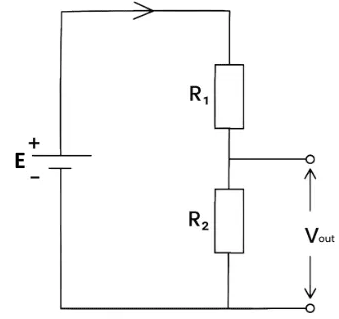
\includegraphics[scale=0.6]{media/Potential Divider.png}
    \caption{A typical circuit diagram for a potential divider.\protect\footnotemark}
\end{figure}
\footnotetext{Source: \url{https://studymind.co.uk/notes/potential-dividers/}}

\begin{proposition}
    The potential difference $V_{\text{out}}$ across $R_2$ is given by \[\frac{V_{\text{out}}}{E} = \frac{R_2}{R_1 + R_2}.\]
\end{proposition}
\begin{proof}
    The current $I$ passing through the resistors is \[I = \frac{E}{R_1 + R_2},\] so the potential difference across $R_1$ is \[V_{\text{out}} = IR_2 = \frac{R_2}{R_1 + R_2} E\] and the desired claim follows.
\end{proof}

\subsection{Potentiometers}

Ideally, when a potential difference is being measure, no current should be drawn from the circuit involved. However, in practice, most voltmeters draw a small current from the circuit.

To remedy this, a \vocab{potentiometer} can be used to compare potential differences without drawing a current from the circuit involved.

\begin{definition}
    A \vocab{potentiometer} is an adjustable potential divider (typically using a sliding contact).
\end{definition}

\begin{figure}[H]
    \centering
    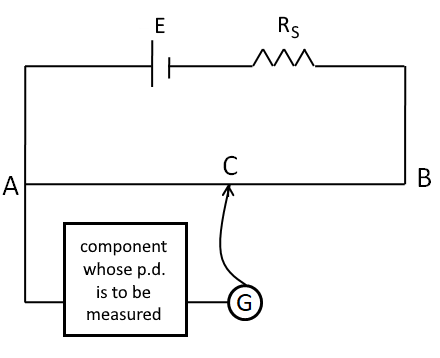
\includegraphics[scale=0.6]{media/Potentiometer Principle.png}
    \caption{A typical potentiometer circuit.}
\end{figure}

For a potentiometer found in laboratories, a length of resistance wire $AB$ is used, acting as two resistors ($AC$ and $CB$). An (optional) additional resistor $R_S$ is connected in series with the wire, serving to limit the current that flows through the circuit. The resistance of $R_S$ will affect the potential difference across $AB$.

A sliding contact is connected to a galvanometer $G$ as shown, and is moved along the wire until a point, $C$, is found on the wire such that there is no current in the galvanometer (null reading). This point is known as the \vocab{null/balance point} and the length $AC$ is known as the \vocab{balance length}. At the null point, the potential difference across $AC$ is equal to the potential difference across the component to be measured. Hence, no current will flow through the galvanometer.

\begin{definition}
    The \vocab{potential gradient} ($\f$) of a potentiometer wire is the potential difference per unit length of the potentiometer wire.
\end{definition}

The SI unit of the potential gradient is volt per metre (V m$^{-1}$).

\begin{principle}[Potentiometer Principle]
    The potential gradient $\f$ of a potentiometer wire is constant, i.e. \[\frac{V_{AB}}{L_{AB}} = \frac{V_{AC}}{L_{AC}} = \f.\]
\end{principle}
\begin{proof}
    Recall that $R = \rho L / A$, so \[\f = \frac{V}{L} = \frac{IR}{L} = \frac{I \rho}{A},\] which is constant.
\end{proof}

\subsubsection{Measuring Electromotive Forces}

To measure the electromotive force of a source, the potentiometer circuit is to be set up as shown below.

\begin{figure}[H]
    \centering
    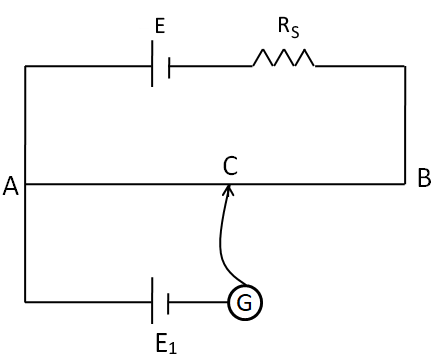
\includegraphics[scale=0.5]{media/Potentiometer Circuit - emf.png}
    \caption{The set-up used to measure the electromotive force of a source using the potentiometer principle.}
\end{figure}

\begin{proposition}
    The electromotive force of the source in the above figure is given by \[\frac{E_1}{E} = \frac{L_{AC}}{L_{AB}} \cdot \frac{R}{R + R_s},\] where $R$ is the resistance of wire $AB$.
\end{proposition}
\begin{proof}
    Let the potential difference across wire $AB$ be $V_{AB}$. Then \[\frac{V_{AB}}{E} = \frac{R}{R + R_S}.\] By the potentiometer principle, \[\frac{E_1}{L_{AC}} = \frac{V_{AB}}{L_{AB}},\] so \[\frac{E_1}{E} = \frac{L_{AC}}{L_{AB}} \cdot \frac{V_{AB}}{E} = \frac{L_{AC}}{L_{AB}} \cdot \frac{R}{R + R_S}.\]
\end{proof}

\subsubsection{Measuring Internal Resistance}

To determine the internal resistance of a source, the potentiometer circuit is to be set up as shown below.

\begin{figure}[H]
    \centering
    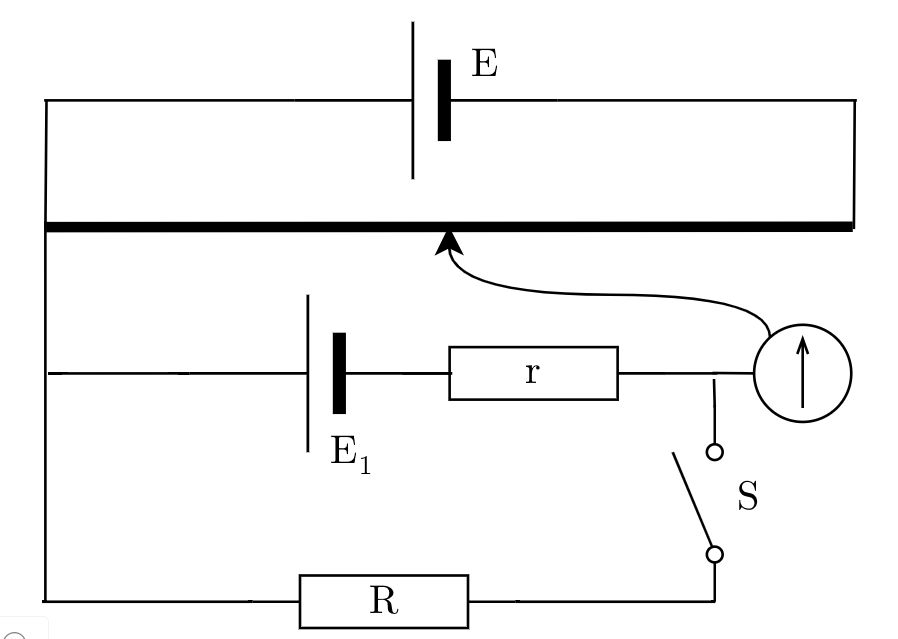
\includegraphics[scale=0.3]{media/Potentiometer Circuit - Internal Resistance.png}
    \caption{The set-up used to measure the internal resistance of a source using the potentiometer principle.}
\end{figure}

\begin{proposition}
    The internal resistance of the cell is given by \[\frac{r}{R} = \frac{L_1}{L_2} - 1,\] where $L_1$ and $L_2$ are the balance lengths when switch $S$ is open and closed respectively.
\end{proposition}
\begin{proof}
    When switch $S$ is open, no current passes through the branch circuit, hence the potential difference across the branch circuit comes solely from the electromotive force $E_1$. Thus, \[\f = \frac{E_1}{L_1}.\]

    When switch $S$ is closed, we can treat the potentiometer as a potential divider. We previously derived that \[\frac{V}{E_1} = \frac{R}{R + r},\] where $V$ is the terminal potential difference. On the other hand, \[\f = \frac{V}{L_2}.\]

    Hence, by the potentiometer principle, \[\frac{E_1}{L_1} = \frac{V}{L_2} \implies \frac{R}{R + r} = \frac{V}{E_1} = \frac{L_2}{L_1} \implies \frac{r}{R} = \frac{L_1}{L_2} - 1.\]
\end{proof}